\chapter{Towards an EU cyber strategy?}

After exploring the concepts essential to develop a coherent approach for our analysis, this section will dive into the role of the European Union (EU) as a cyber actor. The analysis highlights how academic literature observes the EU’s role and identifies critical issues that emerge in its cyber posture. As mentioned in the previous section, securitization is a fundamental aspect of cybersecurity. Since 1957, the EU has played a significant political and economic role in the international arena. Despite the failure of the treaty to establish the European Defence Community and the increasing dominance of NATO, the EU lost its initiative to become more militarily active until the outbreak of the war in Ukraine. Furthermore, the EU has been a guiding force in the cyber domain, from a regulatory perspective. At the same time, the EU faces challenges in several areas. One such area is the fragmented nature of cybersecurity within the EU, which could have an impact on the coherence of EU policy, since there are different national cyber strategies. The renewed emphasis on cyber defence by the EU in recent times has also highlighted the need to build cyber capabilities in the EU. Despite these challenges, the European Union has a defined diplomatic approach to cyber concerns and offers Member States a tool for retaliation. Lastly, this chapter addresses the issue of institutional overlap between the EU and its Member States. Cyber power differs from other types of power. Although information has been considered one of the ancient types of power (Sun Tzu and Thucydides as examples), cyberspace has created a new domain of confrontation in which no geographic borders are present. Thus, the recognition and manifestation of cyber power do not follow the classical theoretical framework.

The EU's concerns about cyber issues became more relevant after the Estonia cyberattack in 2007, leading to the creation of regulations and directives, such as Network and Information Security (NIS) regulation, and the establishment of bodies like the European CyberCrime Centre.


According to Dunn Cavelty (2018), the EU's cyber policy can be divided into three main areas.

\begin{enumerate}
    \item Network and Information Security
    \item Fight against cybercrime
    \item(Military) Cyber Defence and foreign policy 
\end{enumerate}

In this context, the focus will be on the third aspect, which is related to cyber defence and the foreign policy aspects of the EU's cyber power.

The European Union has been considered a success story in the post-1945 era, primarily because of its economic advances and the creation of a single monetary system. However, the Union appears to be less advanced in terms of foreign policy and security. Scholars, such as \textcite{sliwinski_2014_moving}, have been sceptical about the role of the EU, especially in the cybersecurity field. The main critique lies in the intergovernmental nature of the decision-making process behind (cyber) security aspects. According to \textcite{sliwinski_2014_moving}, organisations such as NATO are more suitable as cyber actors because of their real capabilities, adaptiveness, and role in facilitating cooperation, unlike the intergovernmental coordination pursued by the EU. Other authors, such as, \textcite{klimburg_2011_cybersecurity} suggest a division of labour between NATO and the EU in cyberspace. The EU should focus primarily on critical infrastructure protection and develop regulations aiming to harmonise Member States' legislation, mainly regarding the civil aspect. On the other hand, NATO should be more involved in the military aspect of cyberspace, benefiting from the Command and Control (C\&C) advantages within the Atlantic Alliance. This approach reflects the CFSP-NATO relationship.

Furthermore, in recent times, the EU has developed new strategies and capabilities to take concrete action in this direction. For instance, the EU has promoted more standardisation through the establishment of the European Cybersecurity Certification Framework (ECCF) with the EU Cybersecurity Act. This framework affects both the military and civil spheres and aims to enhance cyber capabilities within the EU.

In addition, the cooperation between NATO and the EU has increased on cybersecurity issues. For example, the NATO\textit{ Computer Incident Response Capability} (NCIRC) and the \textit{Computer Emergency Response Team – European Union} (CERT-EU) have been operating daily since 2016 \autocite{eeas_2016_eu}, with the aim of improving cyber incident prevention, detection, and response. NATO-EU cooperation is significantly more advantageous than acting alone, primarily because cyberattacks during peacetime primarily target civil society and critical infrastructure. Additionally, hybrid wars and disinformation campaigns have been conducted within a grey zone, where traditional methods to counteract them are insufficient.

However, during the Russian invasion of Ukraine in 2022, the relationship between NATO and the EU on security issues has developed further, requiring a new investigation to understand the patterns and how it affects the cybersecurity approach of the two organisations in wartime. This work will include this analysis with the aim of filling the gap in cybersecurity cooperation/coordination between the EU and NATO during wartime.

\section{EU Cyber Strategy: an historical perspective on researching resilience and coherence}

The European Union is gradually emerging as a significant player in the cybersecurity domain and aspires to achieve coherence \autocite{carrapico_2017_the}. Assessing the efficiency of EU policies is a challenging endeavour, particularly when applied to novel domains, such as cyberspace. From a theoretical standpoint, enhanced coherence could amplify the effectiveness of EU policies, especially in shared competencies such as cyberspace among Member States. According to \textcite[1256]{carrapico_2017_the}, \textit{coherence can be evaluated through institutional coordination and a shared understanding of security}. Specifically, institutional cooperation is crucial for assessing the development and contribution of institutions to the policy cycle as well as identifying potential overlapping issues, both in terms of political and operational tasks. On the other hand, the shared concept of security enables Member States to develop a comprehensive strategic framework, such as the EU Strategic Compass, facilitating further discussions and integration of security matters.

Since the 1990s, the EU's approach to cybersecurity has undergone a significant evolution, shifting from its initial focus solely on cybercrime to adopting a more comprehensive understanding of cybersecurity. The publication of cybersecurity strategies has played a vital role in promoting coherence within EU actions and preparing a region for future development in this domain. Initially, the EU indirectly addressed cybersecurity concerns by associating the information and technology sector with the Single Market. During the 1990s and the early 2000s, several non-legally binding instruments were approved to counter cybercrimes. Key milestones in this period were the conclusion of the \textit{eEurope 2002 Action Plan, promoting an Information Society for All, and the Commission Communication on Improving the Security of Information Infrastructures and Combating Computer-related Crime (2001)} \autocite{carrapico_2017_the}. However, a significant shift occurred in 2004, prompted by the emerging threat of terrorism, leading the EU to adopt legally binding measures. Simultaneously, in the same year, the \textit{European Network and Information Security Agency} (ENISA) was established to facilitate the exchange of best cybersecurity practices. One notable development was the \textit{Council Framework Decision on Attacks against Information Systems}, which marked a crucial milestone in adopting a transnational approach to cybersecurity within the European Union. This framework is centred on three key pillars: addressing cybercrime, protecting critical information infrastructure (CIIP), and bolstering cyber defence \autocite{carrapico_2017_the}. 

The first document which clearly proposed a strategic approach to the domain was the \textit{EU’s Cybersecurity Strategy} published in 2013. It embedded the three pillars and highlighted the role of the EU in securing economic infrastructure and increasing resilience. According to \textcite{kasper_2021_the}, the new\textit{ EU Cybersecurity Strategy for the Digital Decade}, approved in 2020, highlighted the coherence issue within cybersecurity and other influenced policy areas, conducting steps forward on cyber defence with a more political lens. In this regard, both scholars agree on the EU's ambition to establish itself as a global cyber power, notwithstanding its regional organizational nature. The \textit{NIS Directive (2016/1148)}, the first horizontal legislation on cybersecurity \autocite{markopoulou_2019_the}, constituted a real act on cybersecurity that complies with the EU’s strategy. The directive aims to protect critical infrastructure and IT services from deliberate incidents that can cause disruption. It addresses compliance obligations for addressees and member states' obligations to their respective national strategies and cooperation at the EU level. In this regard, ENISA played a key role in facilitating cooperation between Member States and following the adoption of the NIS Directive in national legislation. The Directive has been updated (2022/2555), affecting a larger group of entities, energy providers or airports, and medium-large enterprises, categorising them between essential and important entities \autocite{enisa_2023_nis}. 

Moreover, \textit{Regulation 2019/881}, also known as the \textit{Cybersecurity Act}, introduced several measures to enhance the EU's cybersecurity capabilities and strengthen its resilience against cyber threats. The Act introduced a comprehensive approach, empowering the European Union Agency for Cybersecurity (ENISA) to coordinate the framework. It allows for voluntary and mandatory cybersecurity certification of ICT products and services, with a focus on critical technologies, through a high-level certification scheme. Additionally, the Act establishes the European Cybersecurity Certification Framework Cooperation Group to ensure the harmonised development and application of certification schemes. Furthermore, it places a strong emphasis on raising cybersecurity awareness and promoting the adoption of certified products and services to enhance the overall cybersecurity posture \autocite{europeanparliament_2019_regulation}. 

\begin{figure}[H]
\centering
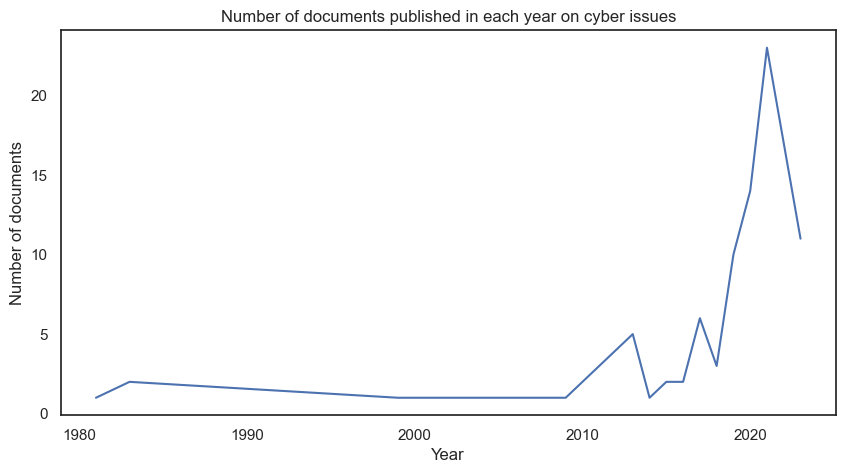
\includegraphics[width=1\textwidth]{Images/eurlex.png}
\caption{\textit{EU Legislation and International Agreements Related to Cyber Issues: 1981 to 2023. The data was retrieved from EUR-Lex. For more information about the keywords used for scraping. For a detailed explanation of the data retrieval process, see Appendix \ref{app:figure_explanation}}}
\label{eurlex.png}
\end{figure}

Over the years, there has been a noticeable increase in the EU's actions concerning cybersecurity. This can be observed through a search on EUR-Lex for legislative and international agreements that encompass cyber-related terms. Notably, there has been a significant surge in publications post-2010, indicating that the EU has elevated cybersecurity to a position of high priority in its policymaking process. All the legislations proposed, embed a multistakeholder approach also reflected in the \textit{EU’s principle of shared responsibility for the effective security of cyberspace} \autocite[6]{christou_2014_the}. The EU has continued to regulate the cyber domain by forging connections with other policy areas, such as the economy, human rights, and security. This integrated approach is crucial for enhancing policy efficiency; however, it requires more institutions to be involved.


\section{Cooperation between institution}

The\textit{Cybersecurity Institutional Map}, created by ENISA, highlights the fragmented and decentralised nature of EU governance on cyber issues. ENISA identifies 18 distinct functions, including R\&D, capacity building, attribution, response to hybrid threats, and the development of cyber resilience. These functions are categorized into four communities: Justice in Cyberspace and Cybercrime Community, Cyber Resilience Community, Cyber Defence Community, and Cyber Diplomacy and Policies Community. Numerous institutions are involved in these diverse responsibilities. The European Agency for Cybersecurity, DG for Communications, CERTs, and EDA are just a few examples that constitute the cybersecurity governance architecture of the EU. Upon initial examination, this hypothesis suggests a potential overlap of functions between several institutions and agencies. As is evident from the Figure \ref{institutional_map.png}, numerous institutions are engaged in similar functions, albeit with varying degrees and scopes. The initial cluster analysis identifies three primary groups: one primarily judicial, another focused on military affairs, and a third encompassing a broader range of functions, which includes the Commission’s DGs and European Agencies, such as The European Defence Agency and ENISA, following the same division between internal and external security issues that have been traditionally applied to European governance \autocite{miadzvetskaya_2021_the}.

\begin{figure}[H]
\centering
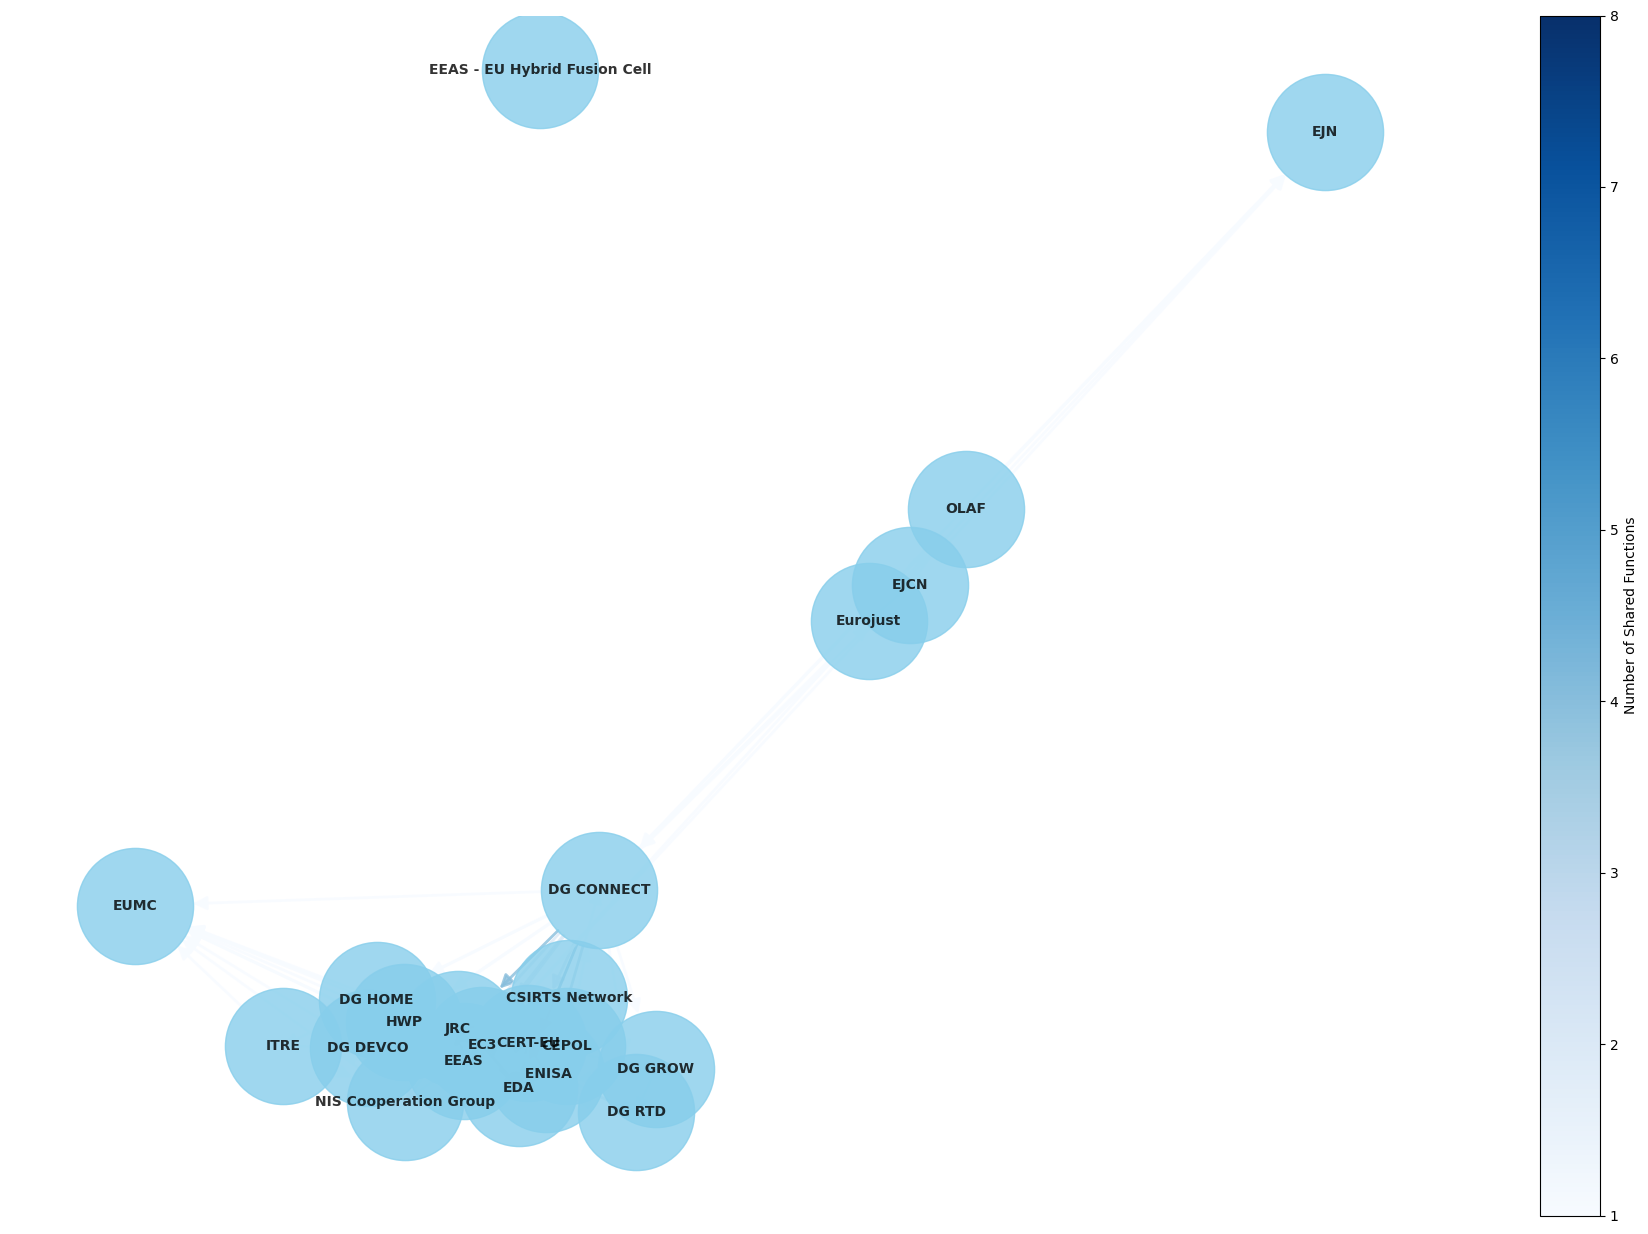
\includegraphics[width=1\textwidth]{Images/institutional_map.png}
\caption{\textit{Clustering ENISA's Cybersecurity Institutional Map showcases EU's diverse institutions collaborating on shared functions in the cyber domain.}}
\label{institutional_map.png}
\end{figure}

\section{Cooperation between Member States}

It is crucial to consider the level of cooperation among Member States in this field, as "despite the increasing Europeanization, cybersecurity in Europe remains solely a national responsibility" \autocite[13]{renard_2014_european}. Several projects at the EU level, such as the \textit{Permanent Structured Cooperation} (PESCO) and initiatives by the European Defence Agency, foster cooperation among participating countries. However, participation in these endeavours remains voluntary, with only a few countries involved. \textcite{kasper_2021_the} emphasizes that \textit{there are no cyber islands} within the EU, highlighting the need for a comprehensive strategy, primarily among EU member states and subsequently with third parties.  The existing literature lacks robust analysis of the EU's role in promoting active cooperation in cybersecurity, largely due to the reasons discussed earlier, as scholars perceive the EU as less capable of enhancing cooperation in the security field compared to other organizations like NATO and OSCE. The concept of EU coherence has some key features to fully understand it. Firstly, there is the prevailing notion that the EU acting as a unitary actor would result in a more \textit{effective} EU. However, this assumption is not inherently evident, particularly in the realm of foreign policy, where the EU has often prioritized unanimity over effectiveness \autocite[5]{missiroli_2001_occasional}. Additionally, it is worth noting that a policy can be effective without necessarily being consistent, as exemplified by metaphors like \textit{carrot-and-stick} or the concept of \textit{good cop-bad cop} \autocite[5]{missiroli_2001_occasional}. Nonetheless, the EU has laid the groundwork and provided a general framework for new instruments that have been increasingly utilized in recent years, such as cyber diplomacy and cyber defence.

\section{Digital Sovereignty}
After the COVID-19 pandemic, the European discourse on resilience and sovereignty has gained greater relevance compared to the past, particularly encompassing various policy areas, including technology and digital domains. The concept of technological sovereignty was first introduced in the 2020 Cybersecurity Strategy and the Strategic Compass, both aimed at promoting the Union's strategic autonomy. However, this idea of sovereignty stands in contrast to the principles of multistakeholder internet governance, which the EU itself supports, emphasizing openness, inclusion, bottom-up collaboration, and consensual decision-making \autocite{pohle_2020_digital}. The EU's perspective on sovereignty revolves around a more political and strategic realm rather than a purely operational one. It perceives cyberspace as a battlefield, where the EU must ensure the security of its citizens against actors, including non-state ones, that challenge the principles of openness and security in the digital arenas. \autocite{andrbarrinha_2022_speaking}. Consequently, the EU has intensified efforts to achieve strategic autonomy in cyberspace through internal and external policies. From an internal standpoint, the EU has introduced risk management-based regulations, exemplified by the NIS Directive and the GDPR \autocite{andrbarrinha_2022_speaking}. On the other hand, the EU has also focused on other policy areas relevant to cyberspace security, investing in strategic sectors.

The European Union and its development since the Treaty of Rome have followed a liberal pathway. It has guaranteed (with different degrees of evolution) the freedom of movement of goods, services, persons and capital. However, globalisation showed new rivals both in economic and political terms. Countries such as China and India have exploited the flourishing European Single Market (ESM) for different purposes: to gain from trade by delocalising their domestic firms and, most important, by investing in those firms that could guarantee the necessary technological know-how. Therefore, the EU guarantees the basis of competition in the ESM (Articles from 101 to 109, TFEU), freedom of establishment in the Union (Articles from 56 to 62, TFEU), and freedom of capital (Article 63, TFEU). Although some barriers have been raised, despite the liberal philosophy accompanying the Union. In the last few years, emerging markets' FDI has affected European strategic sectors. It is dangerous for European stability and integrity when these investments are made by a political (and economic) rival such as China. Consequently, the EU has introduced the \textit{Regulation 2019/452}, designated as the FDI Screening Regulation, as an economic securitisation in a liberal economic context \autocite{shilder_2022_securitisation}. It does not define a new European mechanism for screening foreign investments, but aims to coordinate the Member States. The critical aspect of the Regulation refers only to the security and public aspects of the screening of FDI (Article 1 of Regulation 2019/452), similar to how the Member States may restrict the free movement of capital from third countries (Article 65, TFEU) and regarding hostile investments (Article 207, para.2, TFEU). The economic terms are completely excluded for not undermining the liberal principle of the Union. The Court of Justice of the European Union remarked that FDI falls within the exclusive competence of the EU, while indirect investments, such as portfolio investments, are shared competence \autocite{cjeu_2015_opinion}. In addition, in the Regulation are listed those sectors that could be strategic for the Member States, such as critical infrastructure, both virtual and physical, critical technologies and their dual use (artificial intelligence, semiconductors, among others), media, energy, and raw material material supply chain. The Regulation refers to the rights of the Member States to protect their vital interests (under Article 346, TFEU). In addition to other regulations, such as the Chip's Act or the AI Act, that proactively impact the securitisation of technological domains by establishing barriers against actors who fail to comply with the EU's values, the pursuit of strategic autonomy has emerged as a catalyst for redefining foreign policy instruments in policy areas that cannot be confined to a defined border between internal and external policies.

\section{Cyber diplomacy of the EU}

The EU cyber diplomacy is aimed at shaping the global cybersecurity landscape according to EU values and interests. As stated by the Council of the EU in its guidelines on external EU cyber capacity building, the EU should focus on cooperating with partner countries and regions as a strategic building block of the EU’s cyber diplomacy efforts to promote and protect human rights, gender digital equality, the rule of law, security, inclusive growth, and sustainable development \autocite{counciloftheeuropeanunion_2018_eu}. This approach explains how the EU cyber diplomacy strategy is more focused on cyber issues that impact societies and economies, rather than a purely security-orientated approach to the problem. However, this strategy has experienced a change in its strategic posture due to the Russian invasion of Ukraine. In fact, the EU highlights in its Strategic Compass the need to \textit{develop the Cyber Diplomatic Toolbox and establish a cyber defence policy in the EU to be better prepared for and respond to cyberattacks} \autocite{eeas_2022_a}. The European Union recognised the need for a concerted diplomatic response to tackle malicious cyber activities, leading to the introduction of the \textit{ Cyber Diplomacy Toolbox} (CDT) in June 2017 \autocite{detomascolatin_2020_si}. The primary objective of the CDT was to establish an effective framework for a united EU diplomatic response, aimed at mitigating and deterring potential aggressors in the cyber domain from undermining the political, security and economic interests of the Union \autocite{counciloftheeuropeanunion_2017_council}. To achieve this goal, the framework involved the imposition of targeted restrictive measures against both entities and individuals engaged in malicious cyber activities. The extent of these measures was adjusted in proportion to different considerations, which included factors such as the size, extent, duration, strength, and consequences of cyber operations.


On 30 July 2020, a significant milestone was achieved when the Council of the European Union unanimously enacted restrictive measures targeting six individuals and three entities affiliated with \textit{Al-Qaeda} and \textit{ISIL} \autocite{counciloftheeuropeanunion_2020_regulation}. These measures were specifically directed toward those who were identified as being accountable for or having direct involvement in a range of cyberattacks perpetrated against the EU Member States. It was the first time that the Cyber Diplomatic Toolbox was used as diplomatic retaliation against individuals and entities involved in cyberattacks. This episode opens the path for a new diplomatic posture in cyberspace, which could lead to a cyber-sanction regime \autocite{moret_2017_the}. The Cyber Diplomatic Toolbox includes a range of diplomatic measures that can be summarised as preventive, stable, cooperative, and restrictive measures \parencite{miadzvetskaya_2021_the, counciloftheeuropeanunion_2017_council}. Preventive measures are the EU initiative to promote \textit{ confidence building measures} (CBSs), including third countries, with the aim of increasing cooperation and dialogue between the parties. The Cooperative measures encompass a diplomatic attitude for a peaceful resolution of the cyber incident. The stability measures refer to the declaration of the EU institutions on the general cyber trends or disruptive ones. Lastly, restrictive measures are proportionate to the scope, scale, and duration of aggressive behaviour in cyberspace \autocite{counciloftheeuropeanunion_2017_council}. To apply the so-called cyber-sanctions, the EU has avoided the \textit{attribution} problem by condemning individuals who were related to a particular cyber operation rather than directly a country \parencite{miadzvetskaya_2021_the, bendiek_2018_the}. 

Even if the securitisation role assumed a prominent role in the EU cyber strategy, it is not disjoined from the EU core values. For this reason, the EU’s relation on (not only) the cyber issue with countries that do not reflect those values (such as China or Russia), is not focused on cooperation, but emphasises them as strategic competitors, while assuming retaliatory behaviour against them. For instance, EU decisions to ban TikTok and to introduce limits to Chinese investment in the crucial sector (such as AI or critical infrastructure, even cyber ones) are just some of many examples of the determinant behaviour of the EU to protect and promote its values. In this regard, the pursuit of the EU’s values, even in the cybersecurity international landscape, represents a clear form of coherence. 

A global cybersecurity posture is characterised by a tendency to externalise EU cybersecurity \autocite{miadzvetskaya_2021_the}. This means that the EU recognises the interconnected nature of cyber threats and understands that effective cybersecurity cannot be achieved in isolation. Instead, the EU actively engages in cooperation and collaboration with other countries and international organisations to collectively address cybersecurity challenges.

According to \textcite{kurowska_2019_the}, the EU’s cyber diplomacy could engage in strategic narrative contestation to shape the cyber governance process more effectively. In addition, the EU has committed itself to the international principle of due diligence in cyberspace and improved the exchange of information with third parties to counter cyberattacks \autocite{bendiek_2018_the}. The due diligence has been promoted by controlling the export of dual-use goods \autocite{bendiek_2018_the}, as happened with the sanctions against Russia after the invasion of Ukraine. \textit{The defence area has been marked by a differentiated approach across the EU, and the cyber domain is no exception}  \autocite[426]{miadzvetskaya_2021_the}. The EU’s unanimity requirement makes it difficult to approve acts that deliberately consider a state as a sponsor for a cyberattack, as reflected in the different foreign policy strategies of the Member States. On the other hand, the European Union has achieved progress even with regard to cyber defence, a different instrument if compared to cyber diplomacy, but with the same goal. 

\section{European Cyber Defence}

Cyber defence has become a top priority for the European Union in recent years due to the rising cyber threats faced by member states.  The EU has introduced several regulations, policy documents, and initiatives to enhance cyber defence capabilities and cooperation among member states. In this scenario, the European Union have enhanced its power as a regulatory actor instead of a pure military one. With the EU Cyber Defence Policy Framework acknowledges cyberspace as the fifth domain of operations, alongside the domains of land, sea, air, and space \autocite{counciloftheeuropeanunion_2018_council}. Building normative blocks through Commission driven policy it has been a benefit for the Union considering that not every EU member has considered the cybersecurity as a top policy priority. 

With the creation of \textit{Joint Cyber Unit} (JCU), a new platform was proposed where EU institution, bodies and members could find a better place to improve operational cooperation, coordination, and information sharing. The JCU is also expected to play a role in the EU's response to cyber threats. The EU's Cybersecurity Strategy for the Digital Decade outlines the main objectives and priorities of resilience, technological sovereignty and leadership, and building operational capacity to prevent, deter, and respond. 

On the military perspective, the \textit{European Union External Action} (EEAS) and the\textit{ European Union Military Staff} (EUMS), have agreed on a military vision and strategy on cyberspace as domain of operation. 
In this document, the integration of cyberspace into crosscutting military domain are considered one of the factor which will impact of the freedom of action during military operation \autocite{eeas_2021_mil}, highlighting the importance of coordination of Command \& Control in the tactical and operational level. Both Diplomatic and Military offices emphasized the use of cyber operations as hybrid warfare and those challenges derived from it, making it difficult to apply standard crisis management plans. 

The vision recognizes that the EU has the capability to accomplish its objectives in the cyberspace domain as it does effectively in other domains of the CSDP missions; it has integrated the operations and missions establishing consistent cyber resilience and deterrence as well as established an integrated EU civili-military synergies in \textit{EU Common Security and Defence Policy} (CSDP).  The key takeaways of this strategic document are the capacities and capabilities needed to affirm EU Cyber Strategy under the CSDP. This comprehensive strategy encompasses various dimensions, including cultural adoption, operational capabilities, crisis planning, and international cooperation, with the overarching goal of establishing a stable and secure cyberspace for EU CSDP military operations and missions.

At its core, the strategy acknowledges that adversaries frequently operate below the threshold of armed aggression. This recognition propels the need for continuous adaptation to the evolving cyber threat landscape, marking a strategic shift towards resiliency, defensive actions, and deterrence. Understanding adversarial cyberspace operations as strategic campaigns becomes paramount, emphasizing a holistic cultural adoption that permeates through all levels of EU CSDP military operations. To operationalize this cultural shift, the strategy introduces a coordination and transition instrument as a key facilitator for implementing Cyberspace Operations capabilities. It calls for active involvement from EU institutions, Framework Nations, Member States, and partners. The rapid reflection of capabilities identified through the EU Capability Development Process (CDP) is essential, ensuring that the EU military remains agile in integrating new technologies and methodologies. Along with EU Member States, NATO remains a critical partner on developing a coherent cyber strategy. The partnership goes beyond the cooperation between Computer Incident Response Teams, including cooperation in technology acceleration programs such as \textit{DIANA}. 

From a regulatory perspective, the strategy implies adopting a regulation similar to NIS in the military field. This would result in comprehensive crisis management and interoperability across EU member states, facilitated by collaboration with ENISA.

The document also focusses on the informational gathering. It emphasizes the need for a permanent and federated cyber information sharing and fusion framework, complemented by appropriate processes and technical capabilities, highlighting once again the problem with the information sharing, even through partner actors.

Furthermore, the personnel and skills investment are considered the operational core of the strategy. The development of the Cyberspace\textit{ Education, Training and Exercise} (ETE) at all levels constitutes the core capability of EU cyber defence. As the war in Ukraine demonstrated, the operational skills are the pivotal aspect that involves both defence and offence during cyber operations. Even though the scope could be different (destructive, intelligence gathering, cyber defence or others), the skills to achieve the objective are not so different \autocite{slayton_2017_what}.  

Moreover, collaboration with industry, academia, and the cybersecurity market is emphasized for strategic insight and innovation. The strategy encourages the examination and utilization of opportunities with organizations like the  \textit{European Cyber Security Organisation} (ECSO), leveraging external expertise and fostering a collaborative environment.

Referring to the lessons to be learned and state’s power instruments/cyber capacities Table \ref{tab:power-instruments}, the \textit{European Union Military Vision and Strategy on Cyberspace as a Domain of Operations } has included all the issue presented on the Ukraine-Russia War case study. However, the implementation of those strategies and visions is less clear and further research on them is needed to assess if there have been practical step forwards or the document remained on the political discourse without being applied. 

On the other hand, the active engagement of the European Union (EU) in various  Permanent Structured Cooperation (PESCO) projects constitutes a tangible manifestation of the EU's commitment to translating political declarations into actionable strategies for cybersecurity \footnote{Behind the description, few information are availble on the PESCO projects due to their nature. You can find all the PESCO Projects here: https://www.pesco.europa.eu/ }. Among these initiatives, the\textit{ Cyber Ranges Federations} (CRF), coordinated by Estonia, exemplifies a collaborative effort to consolidate national Cyber Ranges, thereby enhancing cyber training, exercises, and research capabilities. The project underscores the EU's recognition of the need for a collective approach to address evolving cyber threats. In a parallel vein, the \textit{Cyber Threats and Incident Response Information Sharing Platform} (CTIRISP), spearheaded by Greece, reflects a strategic move towards more active cyber defence measures. By establishing a platform for sharing cyber threat intelligence among Member States, the initiative acknowledges the imperative of information exchange in fortifying national cyber defence capabilities. This shift towards proactive measures is indicative of a nuanced understanding of contemporary cyber challenges. The \textit{Strategic C2 System for CSDP Missions and Operations} (EUMILCOM), coordinated by Spain, signifies a targeted effort to enhance the command-and-control systems of EU missions globally. The project's modular and scalable approach underscores the EU's commitment to improving military decision-making processes and operational coordination, aligning with the evolving nature of cyber threats and their geopolitical implications Concurrently, the \textit{Electronic Warfare Capability and Interoperability Programme for Future Joint Intelligence, Surveillance and Reconnaissance} (JISR), led by the Czech Republic, underscores the EU's recognition of the importance of electronic warfare capabilities. The project's focus on a comprehensive feasibility study and potential joint concept adoption indicates a strategic approach to addressing gaps in existing electronic warfare capabilities. Lastly, the \textit{Cyber Rapid Response Teams and Mutual Assistance in Cyber Security} (CRRT), coordinated by Lithuania, manifests the EU's commitment to collective cyber resilience and response capabilities. The emphasis on deployable cyber toolkits and the provision of assistance to member states, EU institutions, and CSDP operations aligns with the recognition of the interconnected and collaborative nature of cybersecurity challenges.

\begin{figure}[H]
    \centering
    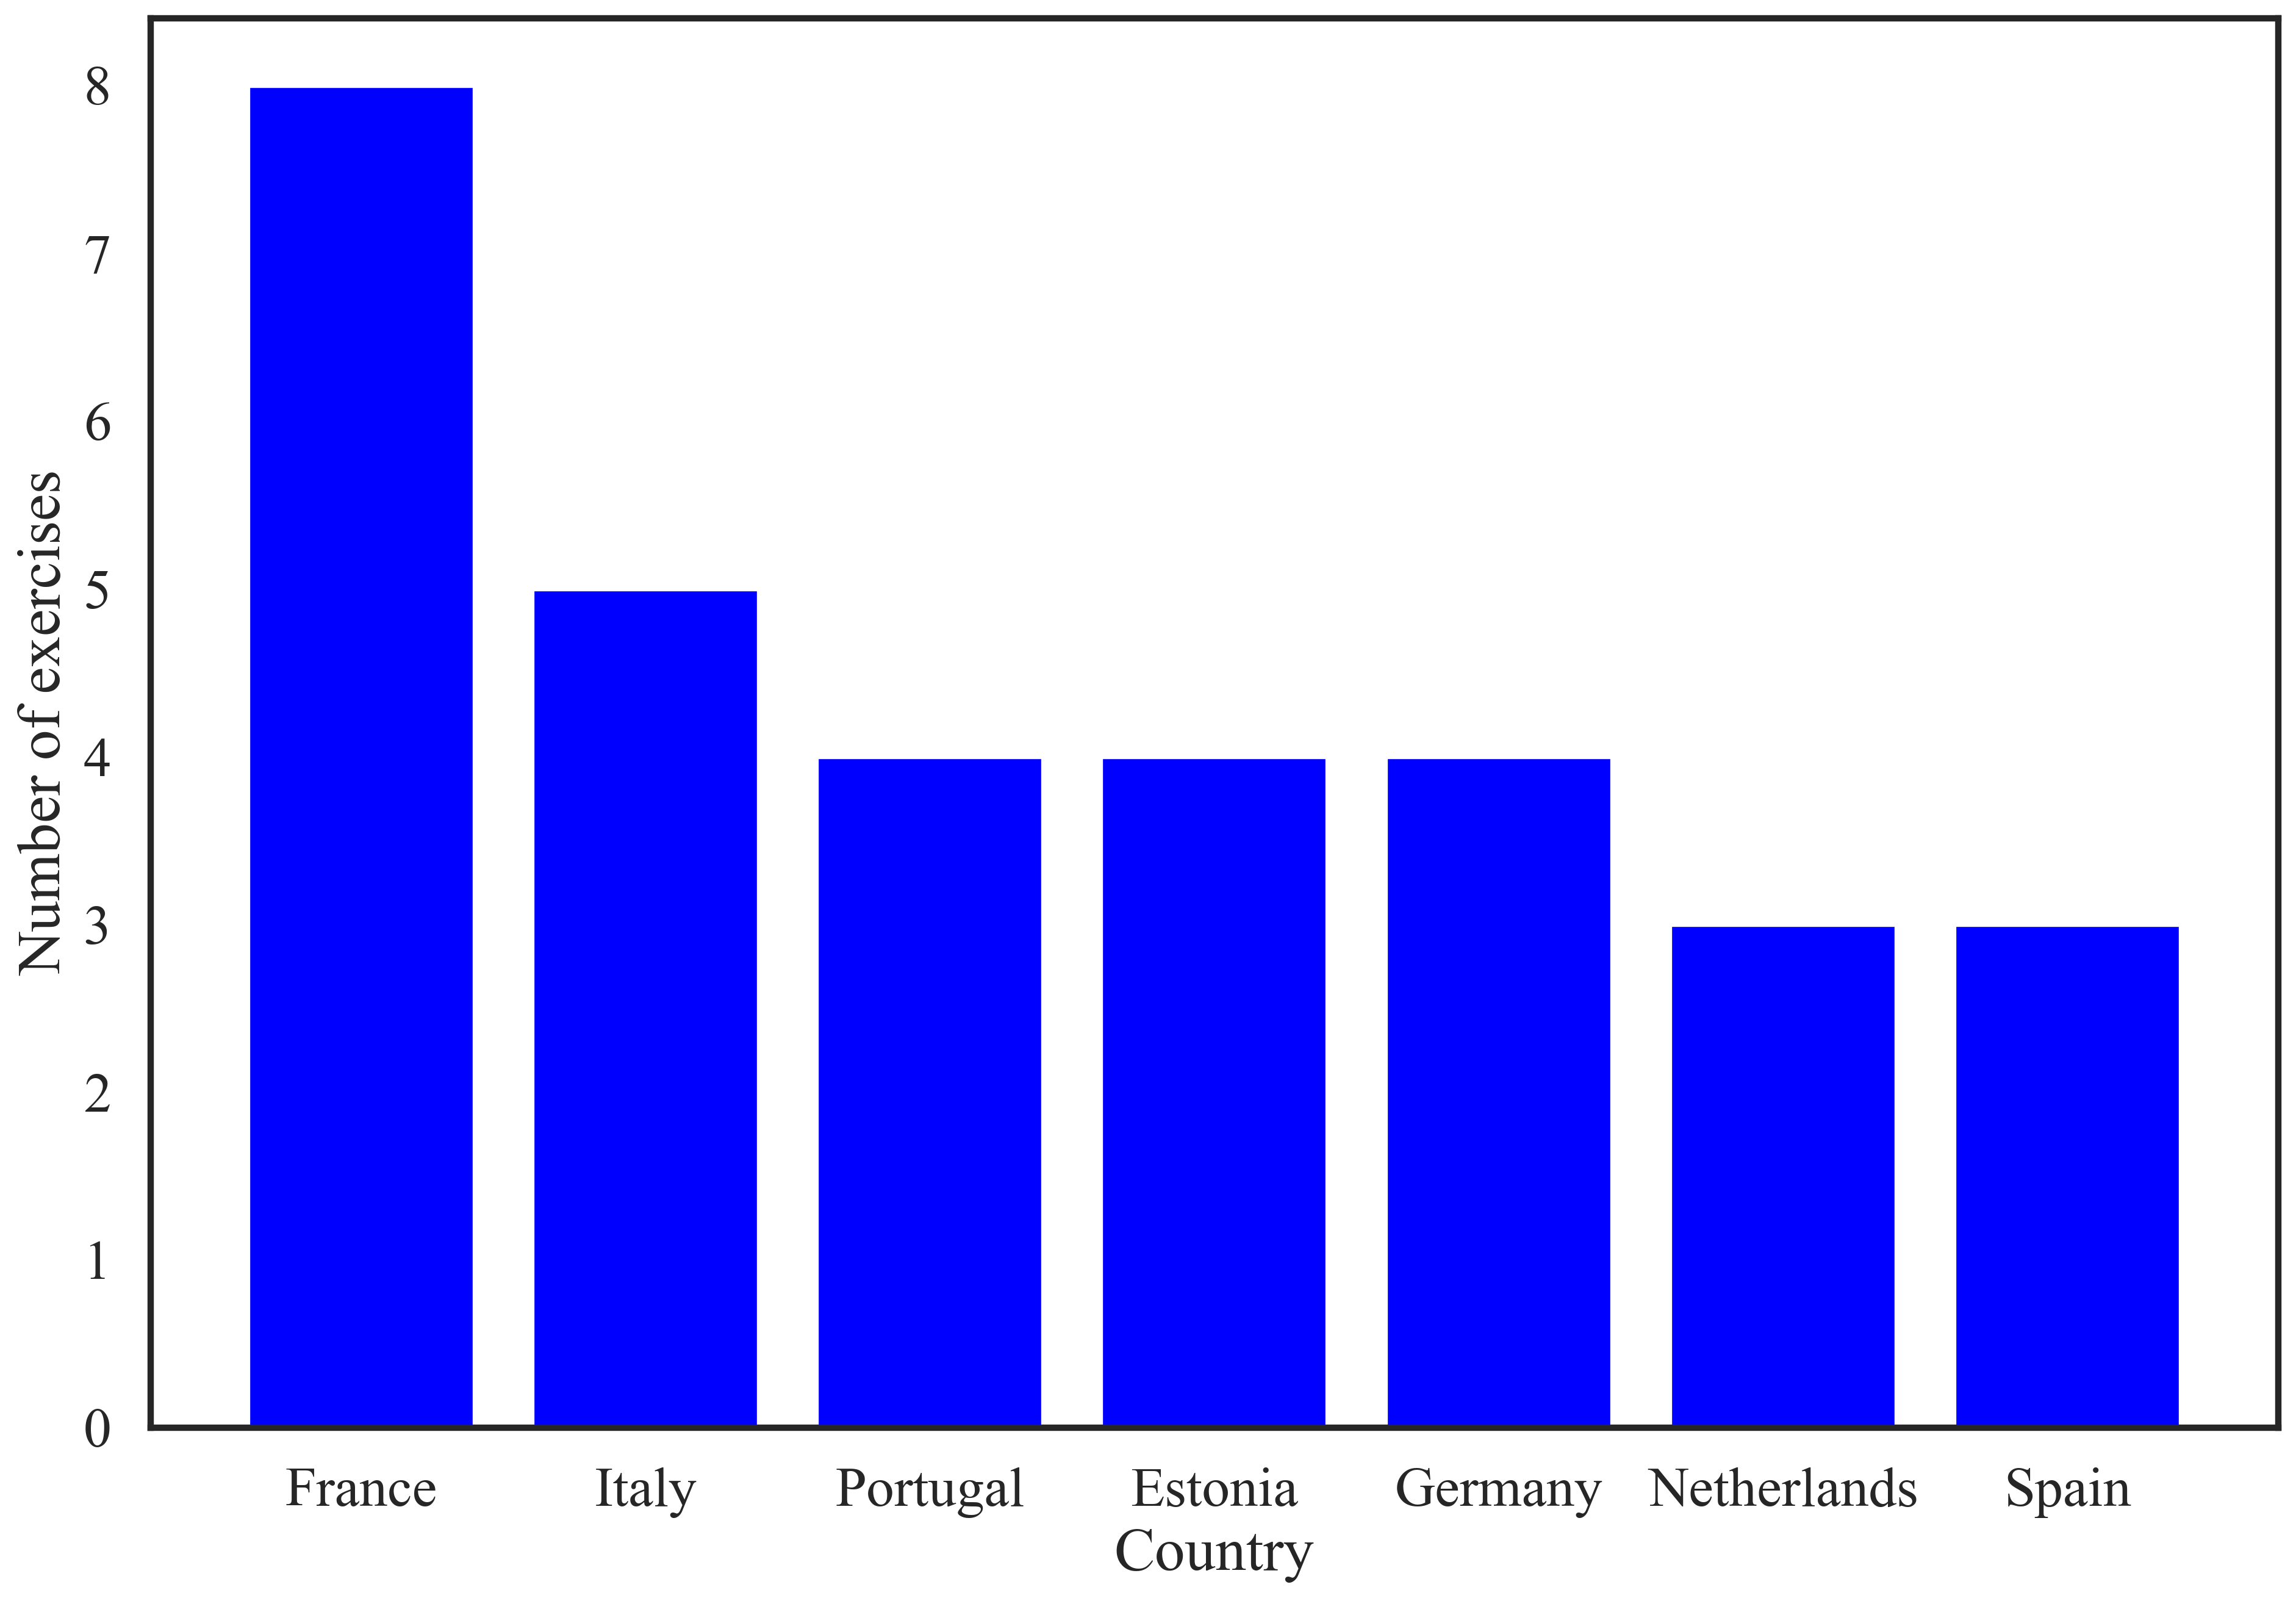
\includegraphics[width=1\textwidth]{Images/cyber_exercises.png}
    \caption{\textit{EU Cyber Projects under PESCO by Country}}
    \source{Source: pesco.europa.eu}
    \label{fig:cyber_exercises}
\end{figure}

Collectively, these PESCO projects represent a concerted effort by the EU to operationalize its cybersecurity objectives, acknowledging the dynamic and multifaceted nature of contemporary cyber threats. The strategic allocation of resources and collaborative approach underscore the EU's commitment to fostering resilience and adaptability in the face of evolving cyber challenges. However, those PESCO missions are just a few examples of missions involved in the cyber domain.

The notable involvement of certain countries in PESCO missions signifies a strategic commitment to collaborative defence initiatives within the European Union. France emerges as a particularly active participant, contributing to eight PESCO projects, showcasing a strong dedication to enhancing European cybersecurity capabilities. Italy closely follows with involvement in five projects, further underlining its commitment to cooperative defence efforts. Portugal, Estonia, and Germany each demonstrate notable engagement, contributing to four projects apiece. The Netherlands and Spain are also actively involved, participating in three projects each. This distribution of involvement suggests a core group of nations taking the lead in shaping the direction and success of PESCO missions. This concentrated participation from key member states contributes to the effectiveness and impact of collaborative cybersecurity endeavours within the European Union.

\section{Conclusion}
The willingness of the European Union to become a cyber power and increase its strategic relevance in the international field is evident. However, the understanding of its cyber capabilities is different from analysing other state-actors. Even though the EU is not primarily involved in military security, the cross-sector nature of cyberspace gives the EU the possibility to emerge as a normative cyber power \autocite{wagnsson_2018_normative}. As a normative cyber power, the EU represent a unified member states perspective while guaranteed the coordination of policies and investment in the cyberspace. Whether this coordination and perspective is and will remain coherent in the future, is the crucial aspect that will define the efficacy of the cyber strategy. 



